%%%%%%%%%%%%%%%%%%%%%%%%%%%%%%%%%%%%%%%%%%%%%%%%%%%%%%%%%%%%%%%%%%%%%%%%%%%%%
\chapter{Analysis of Identity Management}\label{chap:analysis}
%%%%%%%%%%%%%%%%%%%%%%%%%%%%%%%%%%%%%%%%%%%%%%%%%%%%%%%%%%%%%%%%%%%%%%%%%%%%%
\chapterstart

This chapter consists of two parts: the use case and a risk assessment. In the first part a use case is described. The use case tries to picture a typical scenario that requires thoughtful consideration of authentication and authorization technologies depending on the requirements of the use case. Based on the use case a minor risk assessment is done. The risk assessment takes typical threats emerging from authentication and authorization and establishes a risk profile. This risk profile should help to choose an appropriate level of assurance for identity proofing, authentication and federation. 

\section{Use Case}
\label{usecase}
This use case is based on an similar use case of the company "ACP Business Applications" where I am currently employed. This should allow the reader to get a better understanding of the circumstances that led to the design of a federated authentication solution. 

The use case features a medium to large company with up to 1000 employees. The mission of the company is to provide a network and analyzing toolset which allows the customer of the product suite to improve security within his network and keep an overview of potential security risks. Previously the customers received monthly reports about their current state of the network. Each of the products and tools resulted in a separate report which was sent via e-mail. To modernize the approach, the reports should be replaced by a modern single-page application that could be accessed by customers and by employees for administrative reasons. In this example, we call the solution 'Security Assessment Portal.' The Security Assessment Portal should give the customers an overview of current products and the performance of the network. An example of the toolset could be E-Mail-Filtering. The example will be focused on an E-Mail-Filtering-Report and the data which is exposed via the report. It is very important to have a good overview of the data that is used within the application in order to establish appropriate security controls. The Email-Filtering-Report will display a chart per domain. The chart includes data about the amount of e-mails which were blocked, received or carried a virus. 

The company already has a particular set of internal applications that are used by the employees within the company network. The company internally uses active directory for authorization on local machines. All applications until now are accessible within the companies network and are using windows authentication. The application should be accessible by employees as well as customers whereas customers should not receive access to the company network. The data of the customers is sensitive and therefore worth protecting. However it should be kept in mind that because of the sensitive data, certain customer do not want to authenticate with an external provider. The application should be hosted within the company and a solution for customers to access the application from outside is needed. The company needs an authentication solution that meets all the outlined requirements while balancing usability and security. 

The description gives an overview of the company and the expectations for the new application. This leads to the following requirements for the system architecture:

\begin{itemize}
	\item Access from outside the company network is enabled
	\item Application is secured with accounts
	\item Accounts should be managed within the company
	\item Only authenticated users have access to secure contents
	\item Single sign-on for convenience
	\item API for data access
	\item Data can be hosted within the company
	\item The application should be a light weighted Angular solution
\end{itemize} 

The application and its requirements are taken into account in the risk assessment conducted in the next section \ref{riskassessment}. The risk assessment should lead to an better understanding which security measurements are needed for this use case. 

\section{Risk Assessment}
\label{riskassessment}
Risk Assessment is one of the essential elements when it comes to managing risks of an organization. The aim of risk assessment is it to identify, estimate, and prioritize risk to operations, assets, individuals, other organizations and use of the information system. The main task of a risk assessment is to help making decisions on how to respond to certain risk. The steps to a risk assessment are identifying potential threats, internal and external vulnerabilities, the impact to organizations given the potential for threats exploiting vulnerabilities and the likelihood of that harm to occur. There are three tiers according to the 'Guide for Conducting Risk Assessment by NIST (2012) in risk management:

\begin{itemize}
	\item Tier 1 - organizational level
	\item Tier 2 - mission/business process level
	\item Tier 3 - information system level
\end{itemize}

The first two tiers are focusing on risks related to organizational governance and management activities, mission/business processes, enterprise architecture or the funding of information security programs. The third tier focuses more on how to implement a risk management framework successfully [cf. (\cite{NIST:2012:GCRA}, p.1)]. 

The result of the risk assessment should state which assurance levels are appropriate. The available assurance levels are identity proofing assurance level, authentication assurance level and the federate assurance level. Identity proofing assurance level describes the robustness of the process to determine the identity of an individual and should help to avoid identity proofing errors. To determine the robustness of the authentication process and the binding of an authenticator and a specific individual's identifier the authentication assurance level is used. Furthermore choosing an appropriate authentication assurance level should help to avoid authentication errors. The last one of the assurance level is the federated assurance level which is optional since not all identity systems need a federated identity solution. The federated assurance level determines the robustness of the assertion protocol the federation uses to communicate authentication and attribute information and should help to avoid federation errors. All of the assurance levels a described in more detail in the sections \ref{identityProofing} Identity Proofing, \ref{authentication} Authentication and \ref{assertion} Assertion [cf. (\cite{NIST:2017:DIG}, p. 19)]. 

To determine assurance levels one needs to identify the potential risk and which measures exist to minimize the impact of those risks. Two factors are crucial for this task. The first factor is the potential harm or impact, and the second the likelihood of such harm or impact [cf. (\cite{Bolton:2003:EAuth}, pp. 3)]. Bolton (2003), splits harm and impact into these categories:

\begin{itemize}
	\item Inconvenience, distress, or damage to standing or reputation
	\item Financial loss or agency liability
	\item Harm to agency programs or public interests
	\item Unauthorized release of sensitive information
	\item Personal safety
	\item Civil or criminal violations
\end{itemize}

Assurance levels are determined by assessing the potential impact of these categories. The 'Federal Information Processing Standard Publication' by NIST (2004), defines three levels of potential impact concerning security objectives confidentiality, integrity, and availability. Those levels of potential impacts can affect in case of a security breach either the organization or individuals. The levels of impact defined in 'Federal Information Processing Standard Publication' by NIST (2004) are:

\begin{itemize}
	\item Low
	\item Moderate
	\item High
\end{itemize}


If the level is low the loss of confidentiality, integrity or availability has a limited effect. This can mean for example minor damage to organizational assets, short-term inconvenience, short-term distress, short-term embarrassment, limited reveal of personal or sensitive information to unauthorized parties with minor impact, minor financial loss, risk of civil or criminal violation which would not ordinary be subject to enforcement efforts, minor harm to individuals or the capability of the company to fulfill their mission is degraded. If the level of impact is moderate the effects of loss of confidentiality, integrity or availability are serious. Impacts can be significant damage to organizational assets, significant financial loss, serious short-term or limited long-term inconvenience,  serious short-term or limited long-term distress,  serious short-term or limited long-term damage to standing reputation, release of personal or sensitive information to unauthorized parties with moderate impact, risk of civil or criminal violations which may be subject to enforcement efforts, significant harm to individuals or significant degradation of mission fulfillment. The last level of potential impact is high, meaning that the effects can be severe or catastrophic. This means for example major damage to organizational assets, major financial loss, severe or serious long-term inconvenience, severe or serious long-term distress, severe or serious long-term damage to standing reputation, release of personal or sensitive information to unauthorized parties with high impact, risk of civil or criminal violation with special importance to enforcement programs, harm to individuals involving loss of life or serious life-threatening injuries and loss of capability to fulfill the mission [cf. (\cite{NIST:2004:FIOPS}, pp. 6), (\cite{NIST:2017:DIG}, pp. 21)].


The results of the risk assessment are needed to determine the minimum LOA. Once the risk assessment is complete the risk assessment impact profile can then be compared to the impact profiles associated with each assurance level. The table \ref{tab:maxImpacts} can help to determine the required assurance level by finding the lowest level whose impact profile meets or exceeds the potential impact for every category analyzed in the risk assessment [cf. (\cite{NIST:2017:DIG}, p. 25)].

\begin{table}[h]
	\centering
	\begingroup
	\setlength{\tabcolsep}{10pt} % Default value: 6pt
	\renewcommand{\arraystretch}{1.5} % 
	\begin{tabular}{lccc}
		\hline
		\rowcolor[HTML]{656565} 
		{\color[HTML]{FFFFFF} }                                                                                                     & \multicolumn{3}{c}{\cellcolor[HTML]{656565}{\color[HTML]{FFFFFF} Assurance Level}}                  \\ \hline
		\multicolumn{1}{|c|}{\textbf{Impact Categories}}                                                                            & \multicolumn{1}{c|}{\textbf{1}} & \multicolumn{1}{c|}{\textbf{2}} & \multicolumn{1}{c|}{\textbf{3}} \\ \hline
		\multicolumn{1}{|l|}{\begin{tabular}[c]{@{}l@{}}Inconvenience, distress or damage to\\ standing or reputation\end{tabular}} & \multicolumn{1}{c|}{Low}        & \multicolumn{1}{c|}{Mod}        & \multicolumn{1}{c|}{High}       \\ \hline
		\multicolumn{1}{|l|}{Financial loss or agency liability}                                                                    & \multicolumn{1}{c|}{Low}        & \multicolumn{1}{c|}{Mod}        & \multicolumn{1}{c|}{High}       \\ \hline
		\multicolumn{1}{|l|}{Harm to agency programs or public intrests}                                                            & \multicolumn{1}{c|}{N/A}        & \multicolumn{1}{c|}{Low/Mod}    & \multicolumn{1}{c|}{High}       \\ \hline
		\multicolumn{1}{|l|}{Unauthorized release of sensitive information}                                                         & \multicolumn{1}{c|}{N/A}        & \multicolumn{1}{c|}{Low/Mod}    & \multicolumn{1}{c|}{High}       \\ \hline
		\multicolumn{1}{|l|}{Personal safty}                                                                                        & \multicolumn{1}{c|}{N/A}        & \multicolumn{1}{c|}{Low}        & \multicolumn{1}{c|}{Mod/High}   \\ \hline
		\multicolumn{1}{|l|}{Civil or criminal violation}                                                                           & \multicolumn{1}{c|}{N/A}        & \multicolumn{1}{c|}{Low/Mod}    & \multicolumn{1}{c|}{High}       \\ \hline
	\end{tabular}
	\endgroup
	\caption{Maximum Potential Impacts for Each Assurance Level (\cite{NIST:2017:DIG}, p. 25)} \label{tab:maxImpacts}
\end{table}

When analyzing the risk, it should be considered that there could be more than one error and multiple parties could be involved in the process. Furthermore, the potential impacts description often include relative terms like 'minor' and 'serious' which meaning will depend on the context. Over time and with experience the meaning of these relative terms becomes more definite [cf. (\cite{NIST:2017:DIG}, p. 26)].

One of the most useful documents is NIST's 'Guide for Conducting Security Risk assessment'. The guide follows activities related to NIST'S guide of 'Risk Management Framework' which can be either applied to new or legacy information systems. Typically a risk assessment is a very complex task that takes much time and many external sources to be representative, for example expert opinions. If put together correctly one should end up with a Risk Management Framework (RMF). An RMF provides a process that integrates security and risk management activities into the system development life cycle. The system can be applied to both new and legacy systems. 'Risk Management' by NIST (2018) defines 6 Steps in this RMF. The steps include the categorization of the information system, selection of baseline security controls, implementation of security controls, assessment of the security controls, authorize information system operation based on the determination of risk and monitoring security controls. Many industrial standard risk assessment methods across a wide array of fields and industries are based on these guides.  In this practical part, an initial risk assessment is done which should provide a general insight on how to do a risk assessment. The guide to success of a real-life risk assessment is documentation, review, and improvement.  However, since a full RMF is out of scope, a scaled down version that is distinctive of digital identity risk management is conducted  [cf. (\cite{NIST:2018:RMF})].


To prepare for a risk assessment, it helps to identify the purpose, scope, assumptions, and constraints beforehand. The purpose of this risk assessment is to make authorization-related decisions and conducting an initial assessment to identify potential threats, internal and external vulnerabilities which impact the organizations. The scope addresses the 3 Tier -  information system level with a focal point on the risk assessment of a single sign-on federation system. Furthermore, the scope is defined by the result expected from the risk assessment. In this risk assessment, the result should be an authentication and authorization solution for a specific use case. The assessment result should usually be reevaluated after the initial draft. [cf. (\cite{NIST:2012:GCRA}, pp. 24)].

Before starting with the risk assessment a risk model has to be chosen. The model can be translated into risk factors which then can be assessed; these risk factors consist of threat, vulnerability, impact, likelihood and predisposing conditions.  A threat is a circumstance with the potential to impact the organization. Threat events are caused by threat sources. Threat sources that should be considered in the model can address broad threat sources or particular threat sources. Potential threat sources can be adversarial like Insider, Outsider, Trusted Insider, Privileged Insider, Customer, or Competitor. A thread source can also be accidental like User, Privileged User/Administrator or structural like IT-Equipment (Storage, Communication, Processing), Environmental (Temperature/Humidity, Power Supply) or Natural (Fire, Bombing, Earthquake, Sunspots). These potential sources can then cause threat events which can be expressed very general or can also be very specific. Which threat are considered depend highly on the company. A company might choose to only consider previously observed events or all possible events. Examples of potential threat sources are cause integrity loss by injecting false but believable data into organizational information systems, obtain unauthorized access, obtain sensitive data/information from publicly accessible information systems, cause disclosure of critical and/or sensitive information by authorized users, conduct externally-based session hijacking, conduct simple Denial of Service (DoS) attack, craft phishing attacks and so on. The likelihood is a weighted risk factor based on the probability that a given threat is capable of exploring a given vulnerability. A vulnerability is an existing weakness in an information system, system security procedures, internal controls, or implementation that could be exploited by a threat source. Most vulnerabilities are caused by unimplemented or not correctly implemented security controls. Some recommended security controls are described in 'Recommended Security Controls for Federal Information Systems and Organizations'. The implementation of appropriate security controls is an important task that can have a major impact on the operations and assets of a company. Security controls are used to protect the confidentiality, integrity and availability of a system and it's information. Examples are Identifier Management, Authenticator Management or Authenticator Feedback. Closely related to vulnerabilities is a predisposed condition which is a condition within a company which affects the likelihood that threat events once initiated, result in adverse impact on the organization like the involvement of PII. The consequences that a successfully exploited vulnerability by a threat source has, is then described by the impact  [cf. (\cite{NIST:2012:GCRA}, pp. 17, pp. 35, pp. 70), (\cite{NIST:2017:SecurityNPrivacyControls})].

Last but not least before stating a risk assessment based on a risk model, an analytic approach and an assessment approach should be considered. The assessment approach can be quantitative, qualitative or semi-quantitative each of the factors including three assessment scales with different corresponding representations. A quantitative assessment is based on the use of numbers whereas the qualitative assessment typically uses nonnumerical categories or levels like very low, low, moderate, high, very high. Finally, semi-quantitative assessment is a combination of a quantitative and a qualitative assessment using bins, scales or representative numbers. For low impact information systems, the qualitative values are used while for moderate-and high-impact systems; the most granular semi-quantitative values are used. The analysis approach is either threat-oriented, asset/impact-oriented or vulnerability-oriented. With the analysis approach the starting point of the risk assessment can be chosen. The risk assessment starting point can either be based on existing vulnerabilities or assets in the company or possible threats  [cf. (\cite{NIST:2012:GCRA}, pp. 17)].

Based on this knowledge a few examples considering the use case above where conducted. Based on the remarks above and on an example from Hudson (2015) the following steps were followed  'Identify Threat', 'Identify Vulnerability', 'Current Controls', 'Likelihood of Impact', 'Effect of Impact' and 'Risk Determination'. Since it is an initial risk assessment, there are no 'Current Controls'. Therefore, this step is left out. The 'Likelihood of Impact' can be assigned a value from low to high whereas high means it is very likely that a vulnerability is exploited by a threat. The lowest value of 'Likelihood of Impact' is 0.1, and the highest is 1. The 'Effect of the Impact' is assigned a value between 0 to 100. A low 'Effect of Impact' means that the consequences are low and high 'Effect of Impact' means that the consequences are severe. Next to the 'Effect of Impact' of each analysis the associated impact categories are pointed out in order to make it easier to compare the results to the table \ref{tab:maxImpacts}. To determine to the overall risk of a threat, the 'Likelihood' is multiplied with the 'Impact' (Likelihood x Impact) resulting in the risk levels below [cf. (\cite{Hudson:2015:SecurityRisk})]. 

\begin{itemize}
	\item Low =     0-33
	\item Medium = 34-66
	\item High =   67-100
\end{itemize}

Since this analysis is about identity proofing, authentication and federation errors a few threats were chosen to be analyzed with the risk assessment. It should be noted that this does not represent a complete risk assessment since there are more factors to be considered. The risk analysis sees outsiders who want to harm the company and users and identifies them as potential threat sources. 

\paragraph{Identity Proofing Risk 1}

\begin{enumerate}
	\item Technical Threat: An attacker successfully proofs as someone else
	\item Vulnerability: Phishing over unencrypted network communication
	\item Likelihood: 0.5
	\item Impact: 80 (Inconvenience, distress or damage to standing reputation)
	\item \textbf{Risk Determination}: 0.5 x 80 = 40 (Medium Risk) 
\end{enumerate}
\pagebreak[4]

\paragraph{Identity Proofing Risk 2}
\begin{enumerate}
	\item Technical Threat: Collecting and securely storing more information about a person that is required to successfully provide the digital service
	\item Vulnerability: Identity Provider is collecting more information than needed from the user on login. Users might not trust the application or not use it
	\item Likelihood: 0.8
	\item Impact: 30  (Unauthorized release of sensitive information)
	\item \textbf{Risk Determination} : 0.8 x 30 = 24 (Low Risk)
\end{enumerate}


\paragraph{Authentication Risk 1}
\begin{enumerate}
	\item Technical Threat: False claimant using credentials which is not rightfully theirs
	\item Vulnerability: User keeps credentials at an insecure place
	\item Likelihood: 0.9
	\item Impact: 60 (Inconvenience, distress or damage to standing reputation and Unauthorized release of sensitive information )
	\item \textbf{Risk Determination}: 0.9 x 70 = 64 (Medium Risk) 
\end{enumerate}

\paragraph{Authentication Risk 2}
\begin{enumerate}
	\item Technical Threat: Account is compromised and user is using same identifier and authenticator for other accounts
	\item Vulnerability: User uses same credentials for multiply accounts
	\item Likelihood: 0.8
	\item Impact: 70 (Inconvenience, distress or damage to standing reputation and unauthorized release of sensitive information)
	\item \textbf{Risk Determination}: 0.8 x 70 = 56 (Medium Risk)
\end{enumerate}
\pagebreak[4]
\paragraph{Federation Risk 1 }
\begin{enumerate}
	\item Technical Threat: An identity assertion is compromised
	\item Vulnerability: Transaction involving third party not over protected channel
	\item Likelihood: 0.6
	\item Impact: 40 (Inconvenience, distress or damage to standing reputation)
	\item \textbf{Risk Determination}: 0.6 x 40 = 24 (Low Risk)
\end{enumerate}

\paragraph{Federation Risk 2 }
\begin{enumerate}
	\item Technical Threat: Identity Server is unavailable
	\item Vulnerability: Environmental influences 
	\item Likelihood: 0.1
	\item Impact: 100 (Inconvenience, distress or damage to standing reputation and financial loss)
	\item \textbf{Risk Determination}: 0.1 x 100 = 10 (Low Risk)
\end{enumerate}


An initial risk assessment can take a long time but once conducted the following risk assessments will be much quicker. Modern digital services often combine identity proofing, authentication and federation requirements in one single bundle. It is better to look at each of this components separately to delivery the best identity service. The outcome of the separate component can then be compared to categorize of the table \ref{tab:maxImpacts} and which assurance level is associated with the risk outcome. Therefore the highest risk is taken for a category and associated with the appropriate assurance level [cf. (\cite{NIST:2017:DIG}), (\cite{NIST:2018:RMF}), (\cite{Hudson:2015:SecurityRisk})].

\begin{table}[h]
	\centering
	\begingroup
	\setlength{\tabcolsep}{10pt} % Default value: 6pt
	\renewcommand{\arraystretch}{1.5} % 
	\begin{tabular}{lccc}
		\hline
		\rowcolor[HTML]{656565} 
		{\color[HTML]{FFFFFF} }                                                                                                     & \multicolumn{3}{c}{\cellcolor[HTML]{656565}{\color[HTML]{FFFFFF} Assurance Level}}                  \\ \hline
		\multicolumn{1}{|c|}{\textbf{Impact Categories}}                                                                            & \multicolumn{1}{c|}{\textbf{1}} & \multicolumn{1}{c|}{\textbf{2}} & \multicolumn{1}{c|}{\textbf{3}} \\ \hline
		\multicolumn{1}{|l|}{\begin{tabular}[c]{@{}l@{}}Inconvenience, distress or damage to\\ standing reputation\end{tabular}} & \multicolumn{1}{c|}{Low}        & \multicolumn{1}{|c|}{\cellcolor{red!25}Mod}        & \multicolumn{1}{c|}{High}       \\ \hline
		\multicolumn{1}{|l|}{Unauthorized release of sensitive information}                                                         & \multicolumn{1}{c|}{N/A}        & \multicolumn{1}{|c|}{\cellcolor{red!25}Low/Mod}    & \multicolumn{1}{c|}{High}       \\ \hline
	\end{tabular}
	\endgroup
	\caption{Assurance Level Identity Proofing (\cite{NIST:2017:DIG}, p. 25)} \label{tab:identityProofingImpacts}
\end{table}


 To get the suggested assurance level for identity proofing the highest risk determined is relevant. For identity proofing a medium risk was evaluated for 'Inconvenience, distress or damage to standing reputation'. Moreover, for 'Unauthorized release of sensitive information' also a medium risk was evaluated.  According to the table the second LOA is appropriate for identity proofing shown in figure \ref{tab:identityProofingImpacts}.  
 
 \begin{table}[h]
 	\centering
 	\begingroup
 	\setlength{\tabcolsep}{10pt} % Default value: 6pt
 	\renewcommand{\arraystretch}{1.5} % 
 	\begin{tabular}{lccc}
 		\hline
 		\rowcolor[HTML]{656565} 
 		{\color[HTML]{FFFFFF} }                                                                                                     & \multicolumn{3}{c}{\cellcolor[HTML]{656565}{\color[HTML]{FFFFFF} Assurance Level}}                  \\ \hline
 		\multicolumn{1}{|c|}{\textbf{Impact Categories}}                                                                            & \multicolumn{1}{c|}{\textbf{1}} & \multicolumn{1}{c|}{\textbf{2}} & \multicolumn{1}{c|}{\textbf{3}} \\ \hline
 		\multicolumn{1}{|l|}{\begin{tabular}[c]{@{}l@{}}Inconvenience, distress or damage to\\ standing reputation\end{tabular}} & \multicolumn{1}{c|}{Low}        & \multicolumn{1}{|c|}{\cellcolor{red!25}Mod}        & \multicolumn{1}{c|}{High}       \\ \hline
 		\multicolumn{1}{|l|}{Unauthorized release of sensitive information}                                                         & \multicolumn{1}{c|}{N/A}        & \multicolumn{1}{|c|}{\cellcolor{red!25}Low/Mod}    & \multicolumn{1}{c|}{High}       \\ \hline
 	\end{tabular}
 	\endgroup
 	\caption{Assurance Level Authentication (\cite{NIST:2017:DIG}, p. 25)} \label{tab:authenticationImpacts}
 \end{table}
 
The highest risk that were determined for authentication threats are shown in \ref{tab:authenticationImpacts}. For 'Inconvenience, distress or damage to standing reputation' the highest risk determined for authentication is medium. Furthermore, for 'Unauthorized release of sensitive information' it is also medium. Therefore the appropriate assurance level for authentication when comparing the results to categorize of the table \ref{tab:maxImpacts} is the second assurance level. 

Risk determination for federation risks compared to categorize of the \ref{tab:maxImpacts} are shown in table \ref{tab:federationImpacts}. For the category 'Inconvenience, distress or damage to standing reputation' the highest risk evaluated is low and for 'Financial loss or agency liability' the highest risk evaluated is low as well. This leads to an federation assurance level suggestion of one. 

\begin{table}[h]
	\centering
	\begingroup
	\setlength{\tabcolsep}{10pt} % Default value: 6pt
	\renewcommand{\arraystretch}{1.5} % 
	\begin{tabular}{lccc}
		\hline
		\rowcolor[HTML]{656565} 
		{\color[HTML]{FFFFFF} }                                                                                                     & \multicolumn{3}{c}{\cellcolor[HTML]{656565}{\color[HTML]{FFFFFF} Assurance Level}}                  \\ \hline
		\multicolumn{1}{|c|}{\textbf{Impact Categories}}                                                                            & \multicolumn{1}{c|}{\textbf{1}} & \multicolumn{1}{c|}{\textbf{2}} & \multicolumn{1}{c|}{\textbf{3}} \\ \hline
		\multicolumn{1}{|l|}{\begin{tabular}[c]{@{}l@{}}Inconvenience, distress or damage to\\ standing reputation\end{tabular}} & \multicolumn{1}{|c|}{\cellcolor{red!25}Low}        & \multicolumn{1}{c|}{Mod}        & \multicolumn{1}{c|}{High}       \\ \hline
			\multicolumn{1}{|l|}{Financial loss or agency liability}                                                                    & \multicolumn{1}{c|}{\cellcolor{red!25}Low}        & \multicolumn{1}{c|}{Mod}        & \multicolumn{1}{c|}{High}       \\ \hline
	\end{tabular}
	\endgroup
	\caption{Assurance Level Federation (\cite{NIST:2017:DIG}, p. 25)} \label{tab:federationImpacts}
\end{table}


To make it easier to chose an initial assurance level the 'Digital Identity Guidelines' by Grassi, Garcia, \& L. (2017) provide an additional assessment on how to choose a appropriate assurance level. Therefore three flowcharts are provided that need to be followed and will then point to an appropriate assurance level. The flow through the cart is represented with the color red. The first flow chart is figure~\ref{fig:ialflow}. Choosing a Identity Assurance Level however does not mean that the identity proofing has to be done by the party who does the assessment - it can also be federate [cf. (\cite{NIST:2017:DIG})]. 

\begin{figure}[h]
	\centering
	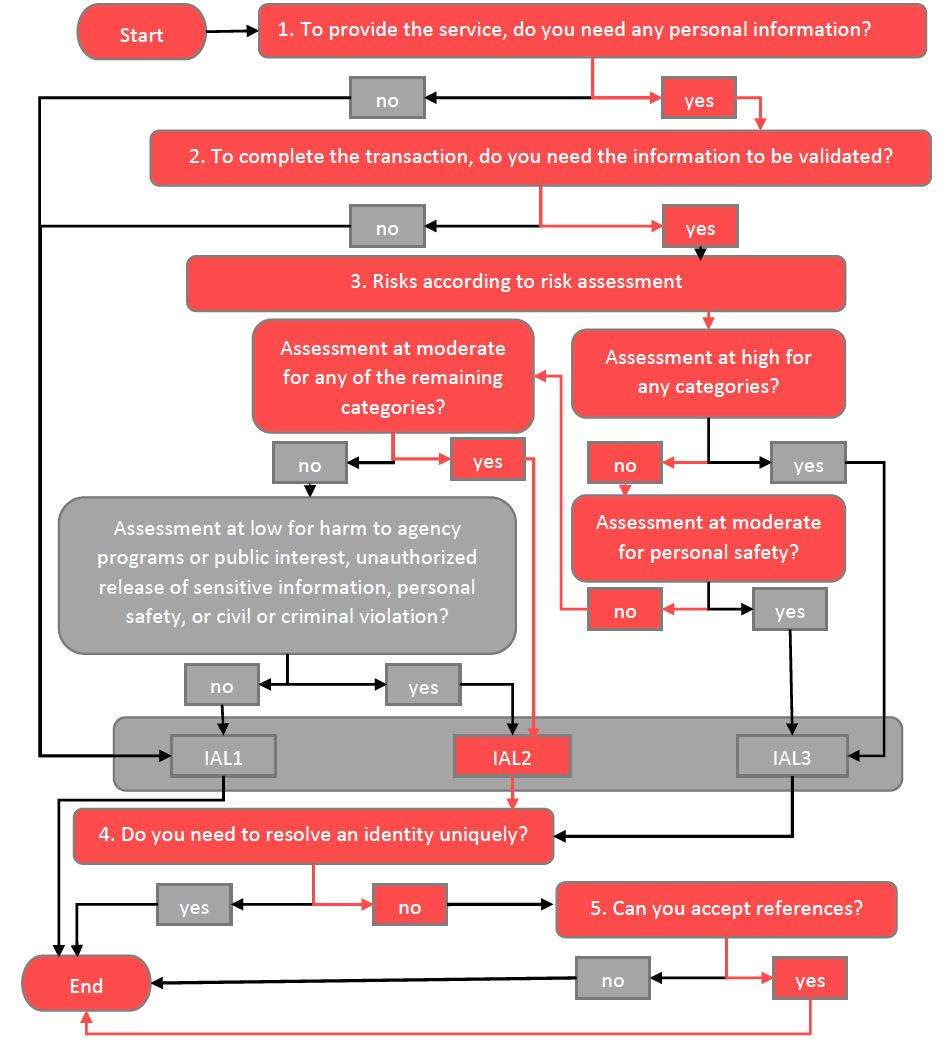
\includegraphics[width=0.9\linewidth]{images/ial_flow_red}
	\caption{Identity Proofing Assurance Flow Chart (\cite{NIST:2017:DIG}, p 27)}
	\label{fig:ialflow}
\end{figure}


In figure~\ref{fig:ialflow} the first question is if PII is needed to provide the service. In our use case, probably sensitive company information is provided therefor yes - personal information is needed. Some of the attributes that are provided have to be validated and can not be self-asserted attributes only therefore the second question can also be answered with - yes.  The next step covers potential impacts of identity proofing. The two threats that is considered here are the most primary identity proofing failures from the view of the user and the company: accepting a falsified identity as true and collecting more information as needed. The before evaluated risks lead to the Identity Assurance Level 2. The two question that are following try to evaluate if a federation is an option. Question four evaluates if the service needs to know the full identity of an user and pseudonymous access even with just a few validated and verified attributes, is not possible. The a answer is no,because in order to reduce the risk of exposure and storing more personal information then necessary a limited set of claims should be accepted. Question five focuses on whether the service should be able to access full attribute values. That does not mean that all attributes have to be delivered in claims, but it should be considered. Since, yes was picked at the question the service is an excellent candidate for a federated infrastructure [cf. (\cite{NIST:2017:DIG}, pp. 28)]. 

\begin{figure}[h]
	\centering
	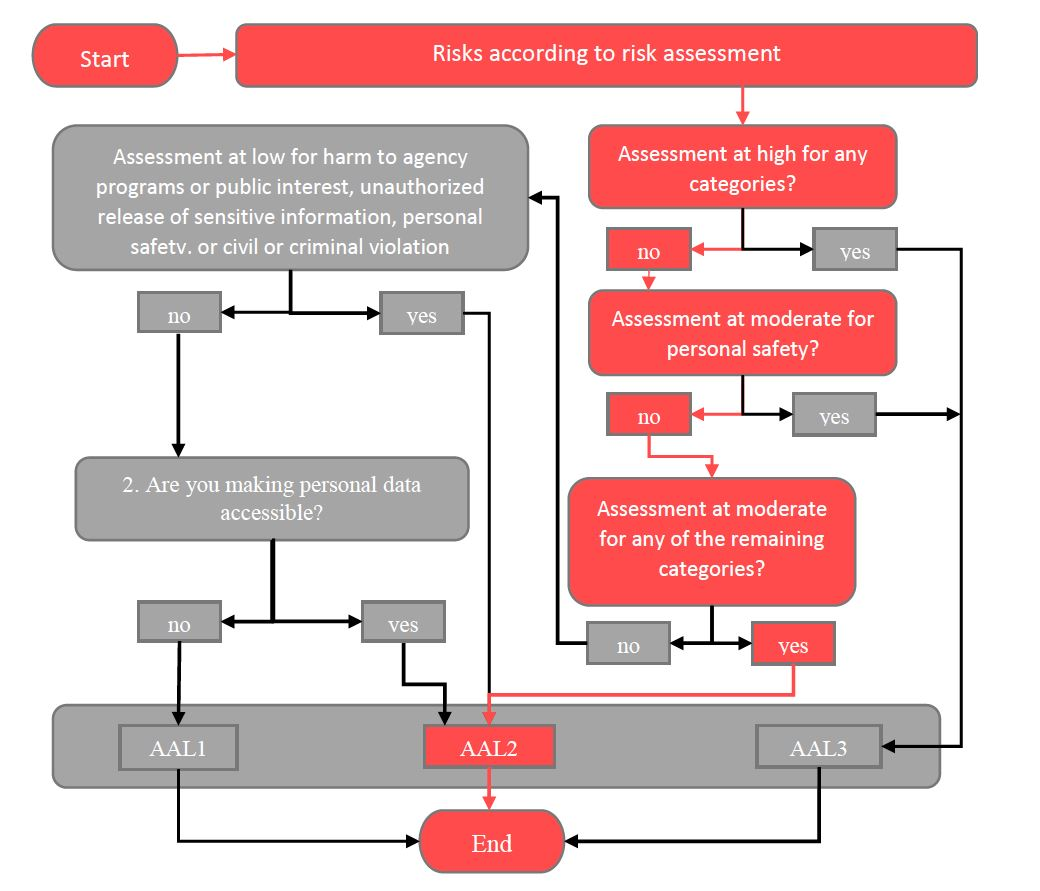
\includegraphics[width=0.9\linewidth]{images/aal_flow_colored}
	\caption{Authentication Assurance Flow Chart (\cite{NIST:2017:DIG}, p 30)}
	\label{fig:aalflow}
\end{figure}

The next flowchart figure~\ref{fig:ialflow} should help to decide on the authenticators necessary for the service. The risks of letting an unauthorized user access information and a compromised account from the risk assessment are taken into account to answer the question. In this use case, sensitive information of the customer are endangered. However, an e-mail filtering report does not have devastating impacts on the customers business, therefore the assessment ends with the AAL2 [cf. (\cite{NIST:2017:DIG}, pp. 30)].  

\pagebreak[4]

\begin{figure}[h]
	\centering
	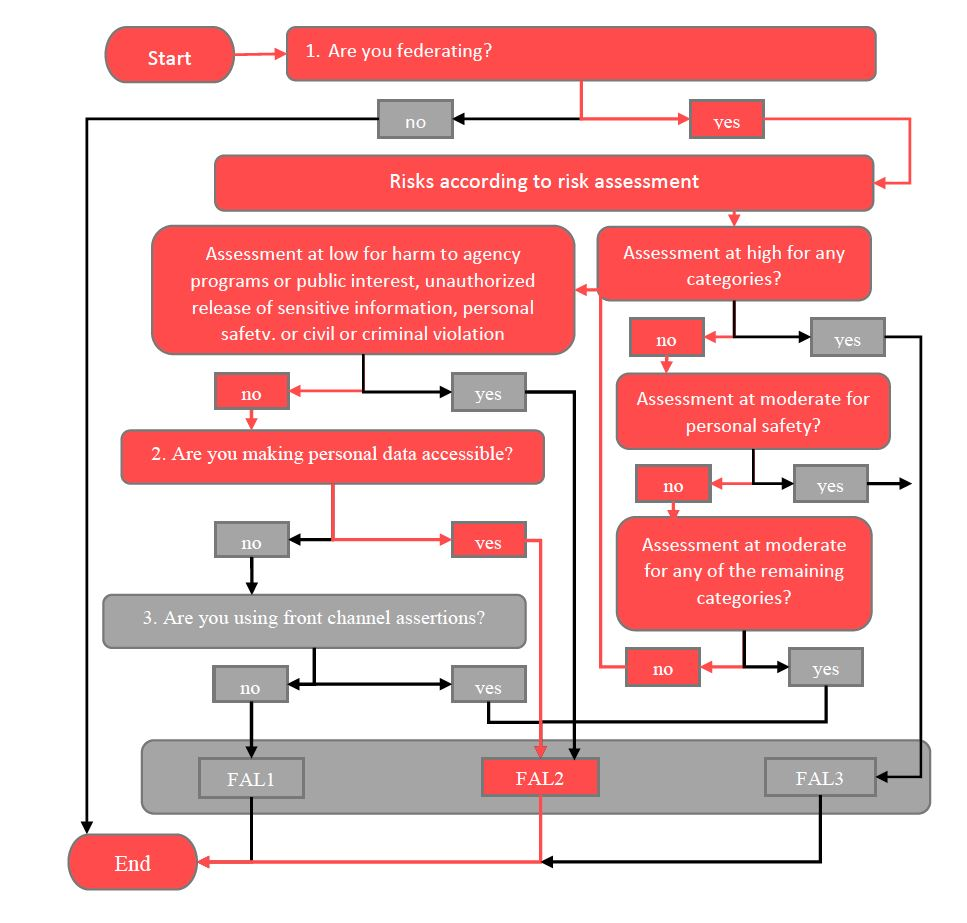
\includegraphics[width=0.9\linewidth]{images/fal_flow_colored}
	\caption{Federation Assurance Flow Chart (\cite{NIST:2017:DIG}, p 32)}
	\label{fig:falflow}
\end{figure}

The last flowchart depicts a federation assurance level flow chart shown in figure~\ref{fig:falflow}. The first question can be answered positivly since a federated service should be considered according to the evaluation in figure~\ref{fig:ialflow}. The next questions are answered according to the conducted risk assessment. This leads to question two, which evaluates if the service will show personal data - yes. The last question leads to Federation Assurance Level 2 [cf. (\cite{NIST:2017:DIG}, pp32)]. 

\pagebreak[4]
\section{Results}
\label{resultSummary}

This initial assertion should give a general direction in which security controls should be in place passed on the different LOA. The risk assessment helps to balance out security and usability, to give the user the best experience possible when using the application. The Risk assessment done in this chapter is based on 'Guide for Conducting Security Risk assessment' by NIST (2012) and on an example done by Hudson (2015). The result indicates which LOA is best suited for the use case presented. The conducted assessment was an initial assessment to create a risk profile. An semi-quantitative assessment approach was used for the assessment and the analysis approach was threat-oriented. The outcomes of this assessment where then compared table \ref{tab:maxImpacts}. After the initial risk assessment with just a view threats that were analyzed the associated assurance level for identity proofing would be \textbf{two}, for authentication risk, it would be \textbf{two}, and for federated risk, the assurance level would be \textbf{one} [cf. (\cite{NIST:2017:DIG}), (\cite{NIST:2018:RMF}), (\cite{Hudson:2015:SecurityRisk})].

Additionally three different flowcharts from were evaluated based on 'Digital Identity Guidelines' by Grassi, Garcia, \& L. (2017). The identity assurance flow chart shown in figure \ref{tab:ial} suggest level \textbf{two} as the right level and indicates that the use case would be a good candidate for federation. The second flowchart shown in figure \ref{tab:aal} also suggest the same level of assurance for authentication as evaluated before - \textbf{two}. Only the last flowchart differs from the previous result. The suggested assurance level for federation is \textbf{two} [cf. (\cite{NIST:2017:DIG})]. 
 
\chapterend
